\documentclass[11pt,a4paper]{article}

% ------------------------------------------------
% COMPATIBILIDAD PDFLATEX
% ------------------------------------------------
\usepackage[utf8]{inputenc}
\usepackage[T1]{fontenc}
\usepackage[spanish, es-tabla]{babel}

% ------------------------------------------------
% FUENTES
% ------------------------------------------------
\usepackage[scaled]{helvet}
\renewcommand{\familydefault}{\sfdefault}

% ------------------------------------------------
% DISEÑO GENERAL
% ------------------------------------------------
\usepackage[a4paper, top=2.54cm, bottom=2.54cm, left=2.54cm, right=2.54cm]{geometry}
\usepackage{tabularx}
\usepackage{titlesec}
\usepackage{enumitem}
\usepackage{fancyhdr}
\usepackage{array}
\usepackage{graphicx} % Necesario para incluir imágenes
\usepackage[hidelinks]{hyperref}

% ------------------------------------------------
% VARIABLES EDITABLES (SOLO CAMBIAR ESTAS DOS)
% ------------------------------------------------
\newcommand{\nombreproyecto}{MUVIOR}
\newcommand{\titulodocumento}{Unidad 3. Actividad 1. Entregable}

% ------------------------------------------------
% ESTILO DE TÍTULOS
% ------------------------------------------------
\titleformat{\section}
  {\normalfont\Large\bfseries}
  {}{0em}{}
\titlespacing*{\section}{0pt}{3ex}{2ex}

% ------------------------------------------------
% ENCABEZADO Y PIE DE PÁGINA
% ------------------------------------------------
\pagestyle{fancy}
\fancyhf{}
\fancyhead[L]{\small \textbf{\nombreproyecto}}
\fancyhead[R]{\small Proyecto de Software I}
\fancyfoot[L]{\small Arquitectura y Diseño}
\fancyfoot[R]{\small J. Carvajal — A00156381 \;|\; F. Franco — A00136798}
\renewcommand{\headrulewidth}{0.4pt}
\renewcommand{\footrulewidth}{0.4pt}

% ------------------------------------------------
% LISTAS
% ------------------------------------------------
\setlist[itemize]{
    noitemsep,
    topsep=0pt,
    leftmargin=1.5em,
    label=\textbullet
}

% ------------------------------------------------
% DOCUMENTO
% ------------------------------------------------
\begin{document}

% ==============================
% PORTADA
% ==============================

\begin{titlepage}
\centering

\vspace*{2.5cm}

{\Huge \textbf{\nombreproyecto}}

\vspace{2.5cm}

\rule{\textwidth}{1.5pt}

\vspace{0.7cm}
{\Huge \textbf{\titulodocumento}}
\vspace{0.7cm}

\rule{\textwidth}{1.5pt}

\vspace{3cm}

\begin{tabularx}{\textwidth}{>{\bfseries}l X}
Institución: & Universidad del Caribe (Unicaribe) \\
Asignatura: & Proyecto de Software I \\
Fecha: & 22 de febrero de 2026 \\
Estado: & Arquitectura y Diseño \\
\end{tabularx}

\vfill

\textbf{Integrantes del equipo}

\vspace{0.5cm}

José Manuel Carvajal Florentino — A00156381 \\
Franklin Franco Quezada — A00136798

\vspace{1.5cm}

22 de febrero de 2026

\end{titlepage}

\newpage

% ==============================
% ÍNDICE
% ==============================

\renewcommand{\contentsname}{Índice de Contenido}
\tableofcontents
\newpage

% ==============================
% PARTE 1: DISEÑO Y CONSTRUCCIÓN
% ==============================

\section{PARTE 1: Diseño y Construcción de la Interfaz}

En esta sección se detallan los elementos visuales y funcionales del proyecto \textbf{\nombreproyecto}, alineando cada captura de pantalla con su descripción técnica correspondiente.

\subsection{1. Pantalla de Bienvenida (Splash)}
\begin{center}
    
\includegraphics[width=0.45\textwidth]{1.png} \\
    \textit{Figura 1: Pantalla de carga con la identidad visual corporativa.}
\end{center}
La aplicación inicia con una pantalla de carga que muestra el isotipo de \nombreproyecto{} en color naranja profundo, estableciendo la paleta de colores oscuro-minimalista desde el primer contacto del usuario.

\subsection{2. Interfaz de Acceso}
\begin{center}
    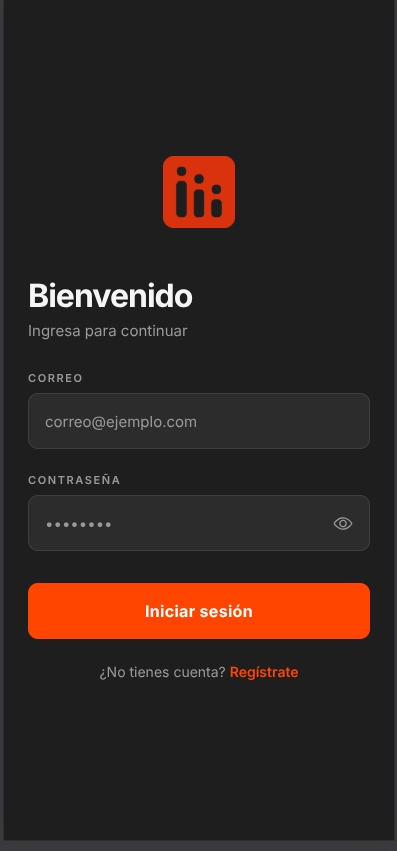
\includegraphics[width=0.45\textwidth]{2.png} \\
    \textit{Figura 2: Formulario de Login para usuarios registrados.}
\end{center}
La pantalla de inicio de sesión presenta campos limpios y validados para el correo y la contraseña. Incluye enlaces directos para el registro de nuevos usuarios bajo el esquema de diseño institucional.

\newpage

\subsection{3. Selección de Perfil (Roles)}
\begin{center}
    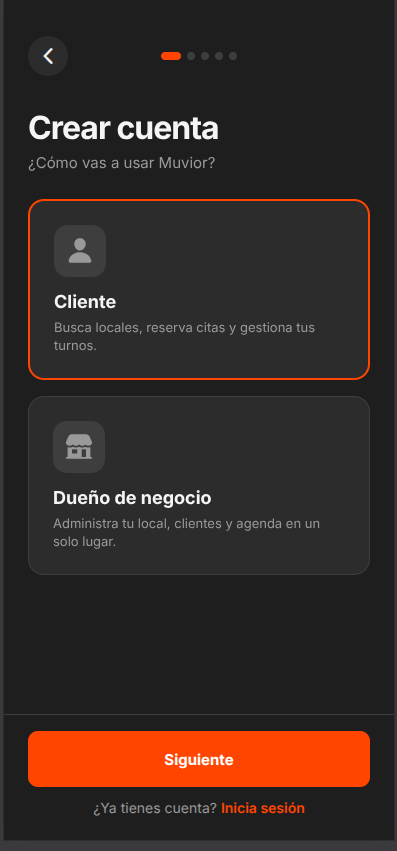
\includegraphics[width=0.45\textwidth]{3.png} \\
    \textit{Figura 3: Selección de tipo de usuario (Cliente o Dueño).}
\end{center}
Durante el registro, el sistema permite al usuario definir si usará la plataforma como \textbf{Cliente} (para buscar locales y tomar turnos) o como \textbf{Dueño de negocio} (para administrar agendamiento y personal).

\subsection{4. Ubicación y Preferencias de Viaje}
\begin{center}
    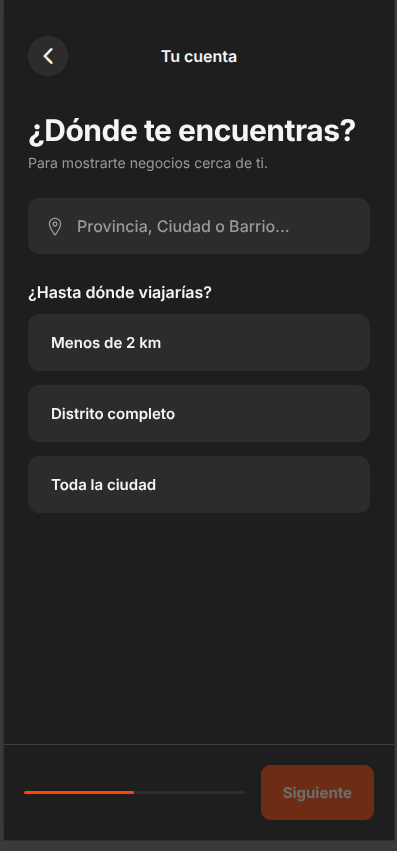
\includegraphics[width=0.45\textwidth]{4.png} \\
    \textit{Figura 4: Selector de radio de búsqueda y zona geográfica.}
\end{center}
Para optimizar las sugerencias, la interfaz solicita la ubicación del usuario y permite configurar qué tan lejos estaría dispuesto a viajar para recibir el servicio.

\newpage

\subsection{5. Pantalla Principal (Dashboard)}
\begin{center}
    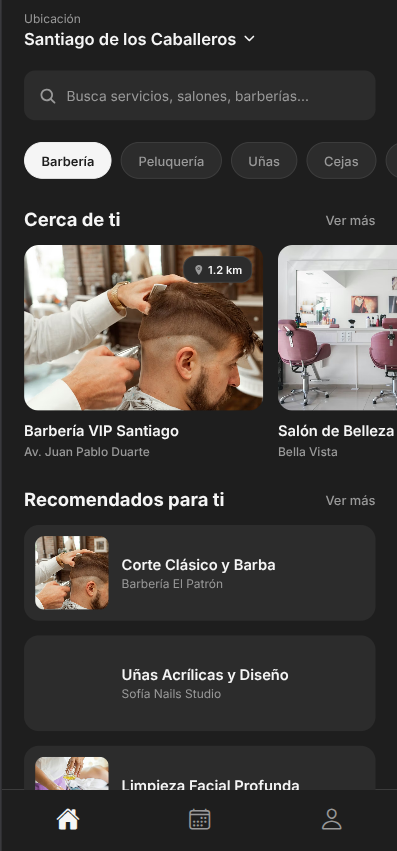
\includegraphics[width=0.45\textwidth]{5.png} \\
    \textit{Figura 5: Exploración de servicios cercanos y recomendados.}
\end{center}
El dashboard central muestra negocios cercanos, servicios recomendados y acceso rápido a categorías principales. Utiliza tarjetas visuales con distancias y nombres descriptivos.

\subsection{6. Configuración de Horario del Local}
\begin{center}
    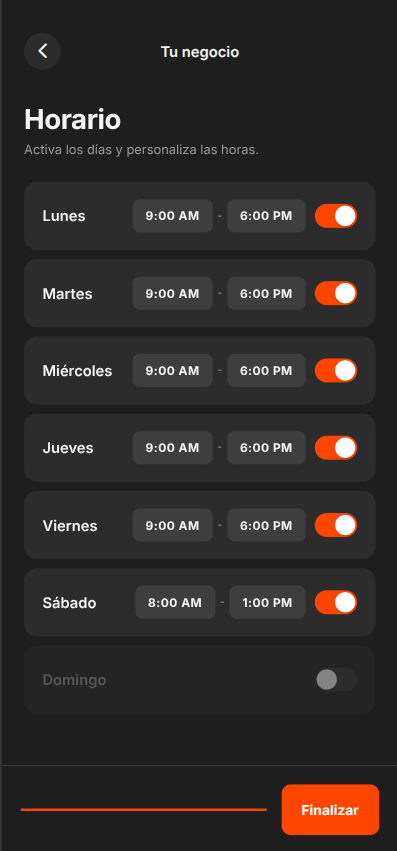
\includegraphics[width=0.45\textwidth]{6.png} \\
    \textit{Figura 6: Gestión de disponibilidad para dueños de negocio.}
\end{center}
Esta interfaz permite a los administradores configurar los días de apertura y las horas de servicio. Es fundamental para que el sistema de turnos solo permita reservas en horarios vigentes.

\newpage

% ==============================
% PARTE 2: GESTIÓN DE TIEMPO
% ==============================

\section{PARTE 2: Gestión de Tiempo del Proyecto (PMBOK)}

Bajo los estándares del \textbf{PMBOK}, se ha definido el plan técnico y la secuencia de actividades necesarias para el desarrollo del software.

\subsection{1. Arquitectura Técnica y Responsabilidades}
\begin{center}
    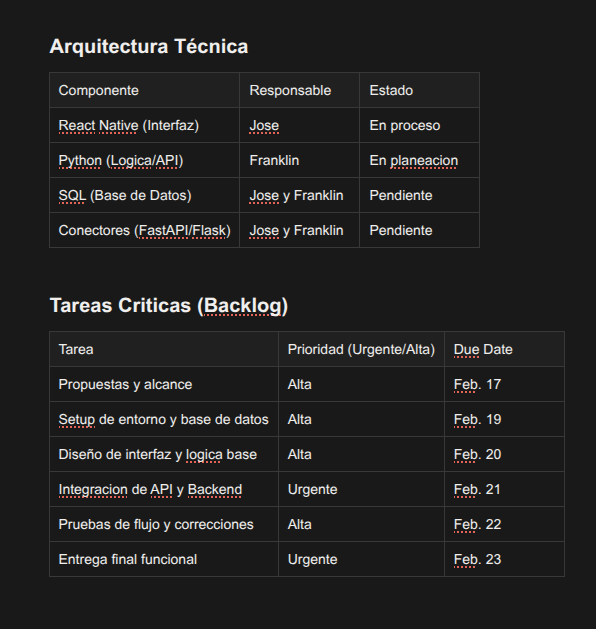
\includegraphics[width=0.8\textwidth]{7.png} \\
    \textit{Figura 7: Tabla de componentes técnicos y backlog de tareas críticas.}
\end{center}
Se ha desglosado el proyecto en componentes (Frontend, Backend, SQL) asignando responsables. El backlog muestra fechas ya cumplidas (Feb. 17-20) y las tareas de integración urgente previstas para el cierre del ciclo.

\subsection{2. Matriz de Procesos y Herramientas}
\begin{center}
    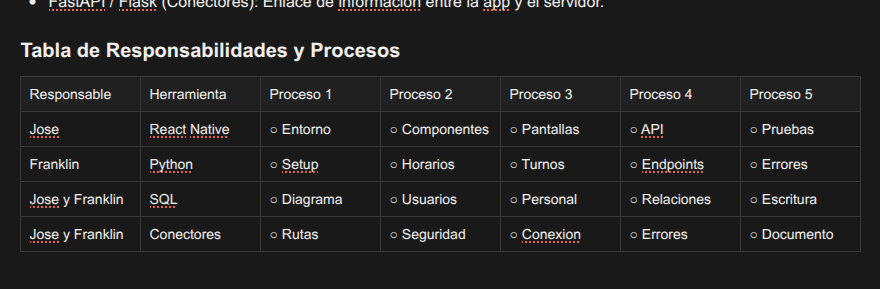
\includegraphics[width=0.9\textwidth]{8.png} \\
    \textit{Figura 8: Tabla de responsabilidades detallada por procesos.}
\end{center}
La gestión del tiempo se apoya en una matriz donde cada integrante del equipo tiene hitos definidos (Proceso 1 al 5). Esto asegura que el desarrollo del entorno, componentes, API y pruebas finales se ejecuten de forma coordinada.

\newpage

\subsection{3. Control del Cronograma}
Se aplicarán revisiones semanales para asegurar que la "Entrega final funcional" se realice en la fecha estipulada (Feb. 23). El uso de herramientas como React Native y FastAPI permite agilizar los tiempos mediante la reutilización de componentes y esquemas de datos.

\end{document}